\Aufgabe[LTL - Monotonicity and Negation Normal Form \hfill\textbf{(2 Point)}]

\begin{enumerate}

\item Let $K_1 = (S, R, L_1)$ and  $K_2 = (S, R, L_2)$ be two Kripke structures with the same set of states $S$ and the same transition relation $R$ such that $L_1(s) \subseteq L_2(s)$ for all states $s \in S$.
    Prove that $K_1,s \models \phi$ implies $K_2,s \models \phi$ for all LTL formulae $\phi$ that do not contain negation.
    \emph{(Hint: prove this statement by structural induction)}.

\item

Exercise 1 defined the \emph{release operator} \textbf{R}.
Prove that the release operator enjoys the following equivalence using the semantics of LTL \emph{(Hint: use the semantics of LTL formulae)}:
\begin{displaymath}
\phi R \psi \equiv \neg (\neg \phi U \neg \psi)
    %\phi \mathbf{R} \psi \equiv \neg(\neg \psi \mathbf{U} \neg \phi)
\end{displaymath}

$$\neg (\neg \phi U \neg \psi)$$


\begin{center}
	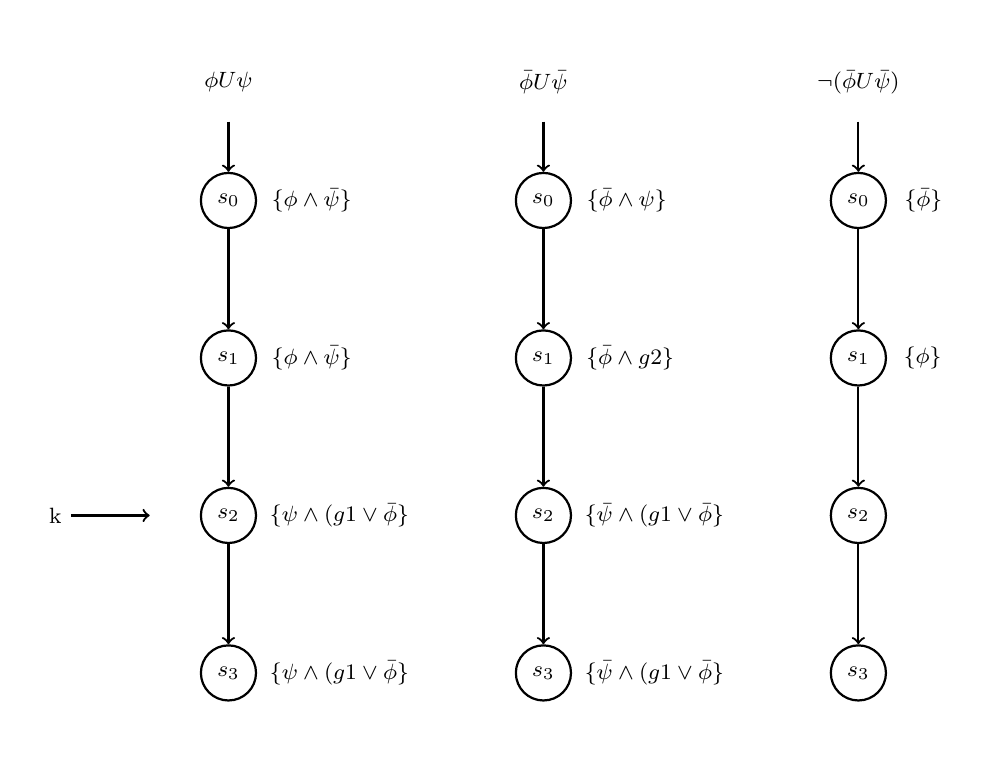
\begin{tikzpicture}[->,scale=1,label distance=0mm]
		\tikzstyle{every node}=[draw,shape=circle,minimum size=7mm,font=\footnotesize];
    \tikzstyle{every path}=[draw,thick];
    \node at (0, 0)   (s0) [label=right:${ \{ \phi  \wedge \bar  \psi  \} }$]  {$s_0$};
    \node at (0, -2)  (s1) [label=right:${ \{ \phi   \wedge \bar  \psi \} }$] {$s_1$};
    \node at (0, -4)  (s2) [label=right:${ \{ \psi   \wedge (g1 \vee \bar  \phi \} }$] {$s_2$};
    \node at (0, -6) (s3) [label=right:${ \{ \psi   \wedge (g1 \vee \bar  \phi \} }$] {$s_3$};
    \draw (0, 1) to (s0);
    \draw (s0) to (s1);
    \draw (s1) to (s2);
    \draw (s2) to (s3);
	\node[draw=none,label=right:{}] at (0,1.5) {$ \phi U \psi $};

	\node at (4, 0)   (sa0) [label=right:${ \{\bar  \phi  \wedge  \psi  \} }$]  {$s_0$};
    \node at (4, -2)  (sa1) [label=right:${ \{\bar  \phi   \wedge g2\} }$] {$s_1$};
    \node at (4, -4)  (sa2) [label=right:${ \{\bar  \psi   \wedge (g1 \vee \bar  \phi \} }$] {$s_2$};
    \node at (4, -6) (sa3) [label=right:${ \{\bar  \psi   \wedge (g1 \vee \bar  \phi \} }$] {$s_3$};
    \draw (4, 1) to (sa0);
    \draw (sa0) to (sa1);
    \draw (sa1) to (sa2);
    \draw (sa2) to (sa3);
	\node[draw=none,label=right:{}] at (4,1.5) {$\bar  \phi U\bar  \psi $};

	\node at (8, 0)   (sb0) [label=right:${ \{\bar  \phi \} }$]  {$s_0$};
    \node at (8, -2)  (sb1) [label=right:${ \{ \phi \} }$] {$s_1$};
    \node at (8, -4)  (sb2) {$s_2$};
    \node at (8, -6) (sb3) {$s_3$};
    \draw (8, 1) to (sb0);
    \draw (sb0) to (sb1);
    \draw (sb1) to (sb2);
    \draw (sb2) to (sb3);
	\node[draw=none] at (8,1.5) {$ \neg (\bar  \phi U\bar  \psi )$};

	\node[draw=none] at (-2.2,-4) {k};
	\draw (-2,-4) to (-1,-4);  
	\end{tikzpicture}
\end{center}

\item

An LTL formula in \emph{negation normal form}, if
\begin{itemize}
\item all negations appear only in front of the atomic propositions,
\item only the logical operators \emph{true}, \emph{false}, $\vee$, and $\wedge$ are used, and
\item only the temporal operators \textbf{X}, \textbf{U}, and \textbf{R} are used.
\end{itemize}

Show that every LTL formula $\phi$ can be transformed into an equivalent formula $\psi$ that is in negation normal form.
\emph{(Hint: prove this statement by structural induction)}.

\end{enumerate}